% Options for packages loaded elsewhere
\PassOptionsToPackage{unicode}{hyperref}
\PassOptionsToPackage{hyphens}{url}
\PassOptionsToPackage{dvipsnames,svgnames,x11names}{xcolor}
%
\documentclass[
  ignorenonframetext,
]{beamer}
\usepackage{pgfpages}
\setbeamertemplate{caption}[numbered]
\setbeamertemplate{caption label separator}{: }
\setbeamercolor{caption name}{fg=normal text.fg}
\beamertemplatenavigationsymbolsempty
% Prevent slide breaks in the middle of a paragraph
\widowpenalties 1 10000
\raggedbottom

\usepackage{amsmath,amssymb}
\usepackage{iftex}
\ifPDFTeX
  \usepackage[T1]{fontenc}
  \usepackage[utf8]{inputenc}
  \usepackage{textcomp} % provide euro and other symbols
\else % if luatex or xetex
  \usepackage{unicode-math}
  \defaultfontfeatures{Scale=MatchLowercase}
  \defaultfontfeatures[\rmfamily]{Ligatures=TeX,Scale=1}
\fi
\usepackage{lmodern}
\usetheme[]{AnnArbor}
\usecolortheme{dolphin}
\usefonttheme{structurebold}
\ifPDFTeX\else  
    % xetex/luatex font selection
\fi
% Use upquote if available, for straight quotes in verbatim environments
\IfFileExists{upquote.sty}{\usepackage{upquote}}{}
\IfFileExists{microtype.sty}{% use microtype if available
  \usepackage[]{microtype}
  \UseMicrotypeSet[protrusion]{basicmath} % disable protrusion for tt fonts
}{}
\makeatletter
\@ifundefined{KOMAClassName}{% if non-KOMA class
  \IfFileExists{parskip.sty}{%
    \usepackage{parskip}
  }{% else
    \setlength{\parindent}{0pt}
    \setlength{\parskip}{6pt plus 2pt minus 1pt}}
}{% if KOMA class
  \KOMAoptions{parskip=half}}
\makeatother
\usepackage{xcolor}
\newif\ifbibliography
\setlength{\emergencystretch}{3em} % prevent overfull lines
\setcounter{secnumdepth}{-\maxdimen} % remove section numbering


\providecommand{\tightlist}{%
  \setlength{\itemsep}{0pt}\setlength{\parskip}{0pt}}\usepackage{longtable,booktabs,array}
\usepackage{calc} % for calculating minipage widths
\usepackage{caption}
% Make caption package work with longtable
\makeatletter
\def\fnum@table{\tablename~\thetable}
\makeatother
\usepackage{graphicx}
\makeatletter
\def\maxwidth{\ifdim\Gin@nat@width>\linewidth\linewidth\else\Gin@nat@width\fi}
\def\maxheight{\ifdim\Gin@nat@height>\textheight\textheight\else\Gin@nat@height\fi}
\makeatother
% Scale images if necessary, so that they will not overflow the page
% margins by default, and it is still possible to overwrite the defaults
% using explicit options in \includegraphics[width, height, ...]{}
\setkeys{Gin}{width=\maxwidth,height=\maxheight,keepaspectratio}
% Set default figure placement to htbp
\makeatletter
\def\fps@figure{htbp}
\makeatother
% definitions for citeproc citations
\NewDocumentCommand\citeproctext{}{}
\NewDocumentCommand\citeproc{mm}{%
  \begingroup\def\citeproctext{#2}\cite{#1}\endgroup}
\makeatletter
 % allow citations to break across lines
 \let\@cite@ofmt\@firstofone
 % avoid brackets around text for \cite:
 \def\@biblabel#1{}
 \def\@cite#1#2{{#1\if@tempswa , #2\fi}}
\makeatother
\newlength{\cslhangindent}
\setlength{\cslhangindent}{1.5em}
\newlength{\csllabelwidth}
\setlength{\csllabelwidth}{3em}
\newenvironment{CSLReferences}[2] % #1 hanging-indent, #2 entry-spacing
 {\begin{list}{}{%
  \setlength{\itemindent}{0pt}
  \setlength{\leftmargin}{0pt}
  \setlength{\parsep}{0pt}
  % turn on hanging indent if param 1 is 1
  \ifodd #1
   \setlength{\leftmargin}{\cslhangindent}
   \setlength{\itemindent}{-1\cslhangindent}
  \fi
  % set entry spacing
  \setlength{\itemsep}{#2\baselineskip}}}
 {\end{list}}
\usepackage{calc}
\newcommand{\CSLBlock}[1]{\hfill\break\parbox[t]{\linewidth}{\strut\ignorespaces#1\strut}}
\newcommand{\CSLLeftMargin}[1]{\parbox[t]{\csllabelwidth}{\strut#1\strut}}
\newcommand{\CSLRightInline}[1]{\parbox[t]{\linewidth - \csllabelwidth}{\strut#1\strut}}
\newcommand{\CSLIndent}[1]{\hspace{\cslhangindent}#1}


% logo
\titlegraphic{
\includegraphics[width=4cm]{000_logos/logo-blue-vertical}}
\logo{\ifnum\thepage>1
\includegraphics[width=0.5cm]{000_logos/logo-blue-vertical}\fi}

% UMNG: Manual de image institucional

% Colors

% Umng
\definecolor{yellow}{HTML}{fdc600}
\definecolor{red}{HTML}{ee2a24}

% Estudios a Distancia
\definecolor{blue1}{HTML}{12245b}
\definecolor{blue2}{HTML}{767ca6}
\definecolor{blue3}{HTML}{cad2ec}

% Modify items
\setbeamercolor{palette primary}{bg=blue3}
\setbeamercolor{palette tertiary}{bg=blue1}
\setbeamercolor{frametitle}{bg=yellow}

% Hyperlinks
\hypersetup{
  linkcolor=red,
  citecolor=red
}

\makeatletter
\@ifpackageloaded{caption}{}{\usepackage{caption}}
\AtBeginDocument{%
\ifdefined\contentsname
  \renewcommand*\contentsname{Table of contents}
\else
  \newcommand\contentsname{Table of contents}
\fi
\ifdefined\listfigurename
  \renewcommand*\listfigurename{List of Figures}
\else
  \newcommand\listfigurename{List of Figures}
\fi
\ifdefined\listtablename
  \renewcommand*\listtablename{List of Tables}
\else
  \newcommand\listtablename{List of Tables}
\fi
\ifdefined\figurename
  \renewcommand*\figurename{Figure}
\else
  \newcommand\figurename{Figure}
\fi
\ifdefined\tablename
  \renewcommand*\tablename{Table}
\else
  \newcommand\tablename{Table}
\fi
}
\@ifpackageloaded{float}{}{\usepackage{float}}
\floatstyle{ruled}
\@ifundefined{c@chapter}{\newfloat{codelisting}{h}{lop}}{\newfloat{codelisting}{h}{lop}[chapter]}
\floatname{codelisting}{Listing}
\newcommand*\listoflistings{\listof{codelisting}{List of Listings}}
\makeatother
\makeatletter
\makeatother
\makeatletter
\@ifpackageloaded{caption}{}{\usepackage{caption}}
\@ifpackageloaded{subcaption}{}{\usepackage{subcaption}}
\makeatother

\ifLuaTeX
\usepackage[bidi=basic]{babel}
\else
\usepackage[bidi=default]{babel}
\fi
\babelprovide[main,import]{english}
% get rid of language-specific shorthands (see #6817):
\let\LanguageShortHands\languageshorthands
\def\languageshorthands#1{}
\ifLuaTeX
  \usepackage{selnolig}  % disable illegal ligatures
\fi
\usepackage{bookmark}

\IfFileExists{xurl.sty}{\usepackage{xurl}}{} % add URL line breaks if available
\urlstyle{same} % disable monospaced font for URLs
\hypersetup{
  pdftitle={Finding and Using Negotiation Power},
  pdfauthor={Luis Francisco Gómez López},
  pdflang={en},
  colorlinks=true,
  linkcolor={Maroon},
  filecolor={Maroon},
  citecolor={Blue},
  urlcolor={Blue},
  pdfcreator={LaTeX via pandoc}}


\title{Finding and Using Negotiation Power}
\author{Luis Francisco Gómez López}
\date{2024-07-26}
\institute{FAEDIS}

\begin{document}
\frame{\titlepage}

\renewcommand*\contentsname{Table of contents}
\begin{frame}[allowframebreaks]
  \frametitle{Table of contents}
  \tableofcontents[hideallsubsections]
\end{frame}

\section{Please Read Me}\label{please-read-me}

\begin{frame}{}
\phantomsection\label{section}
\begin{itemize}
\item
  Check the message \textbf{Welcome greeting} published in the News
  Bulletin Board.
\item
  Dear student please edit your profile uploading a photo where your
  face is clearly visible.
\item
  The purpose of the virtual meetings is to answer questions and not to
  make a summary of the study material.
\item
  This presentation is based on
  (\citeproc{ref-lewicki_negociacion_2024}{Lewicki, Barry, and Saunders
  2024, chap. 8})
\end{itemize}
\end{frame}

\section{Purpose}\label{purpose}

\begin{frame}{}
\phantomsection\label{section-1}
Understand the role of power and the different sources from which this
element arises in a negotiation.
\end{frame}

\section{Power in the context of a
negotiation}\label{power-in-the-context-of-a-negotiation}

\begin{frame}{}
\phantomsection\label{section-2}
\begin{itemize}
\item
  Power in the context of a negotiation refers to the ability of a
  negotiator to gain an advantage or increase the likelihood of
  approaching its target point.
\item
  Power is important in a negotiation because it generates advantages
  and allows reaching a settlement point close to the target point.
\end{itemize}
\end{frame}

\begin{frame}{}
\phantomsection\label{section-3}
\begin{figure}

\centering{

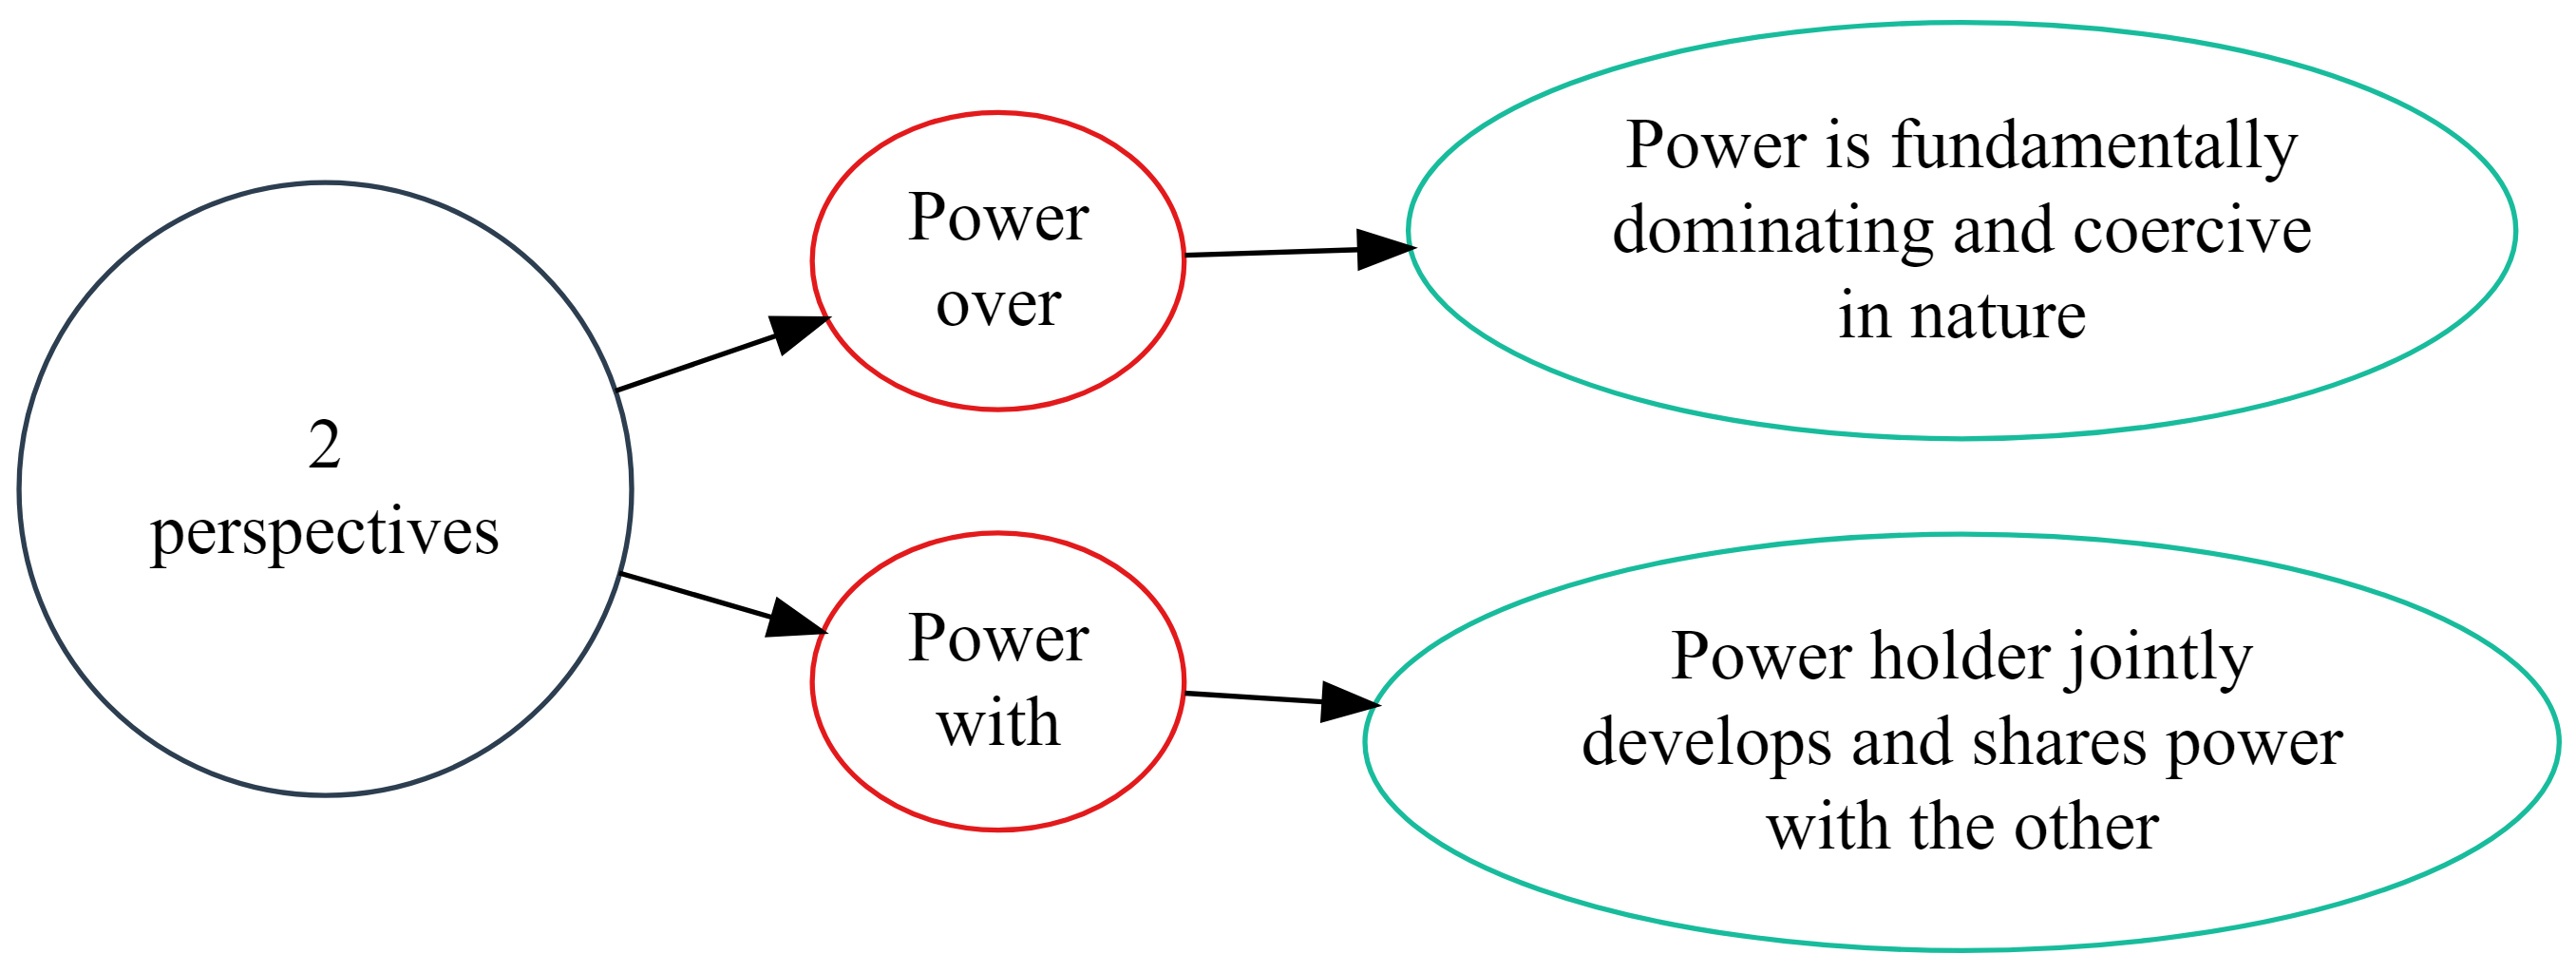
\includegraphics[width=4.5in,height=2.5in]{007_power_files/figure-beamer/dot-figure-1.png}

}

\caption{\label{fig-perspectives-about-power}Perspectives about
power\footnote<.->{Check out (\citeproc{ref-coleman_power_2014}{Coleman
  2014}) if you want a general perspective about power and its relation
  with conflict}}

\end{figure}%
\end{frame}

\section{Sources of power in a
negotiation}\label{sources-of-power-in-a-negotiation}

\begin{frame}{}
\phantomsection\label{section-4}
\begin{figure}

\centering{

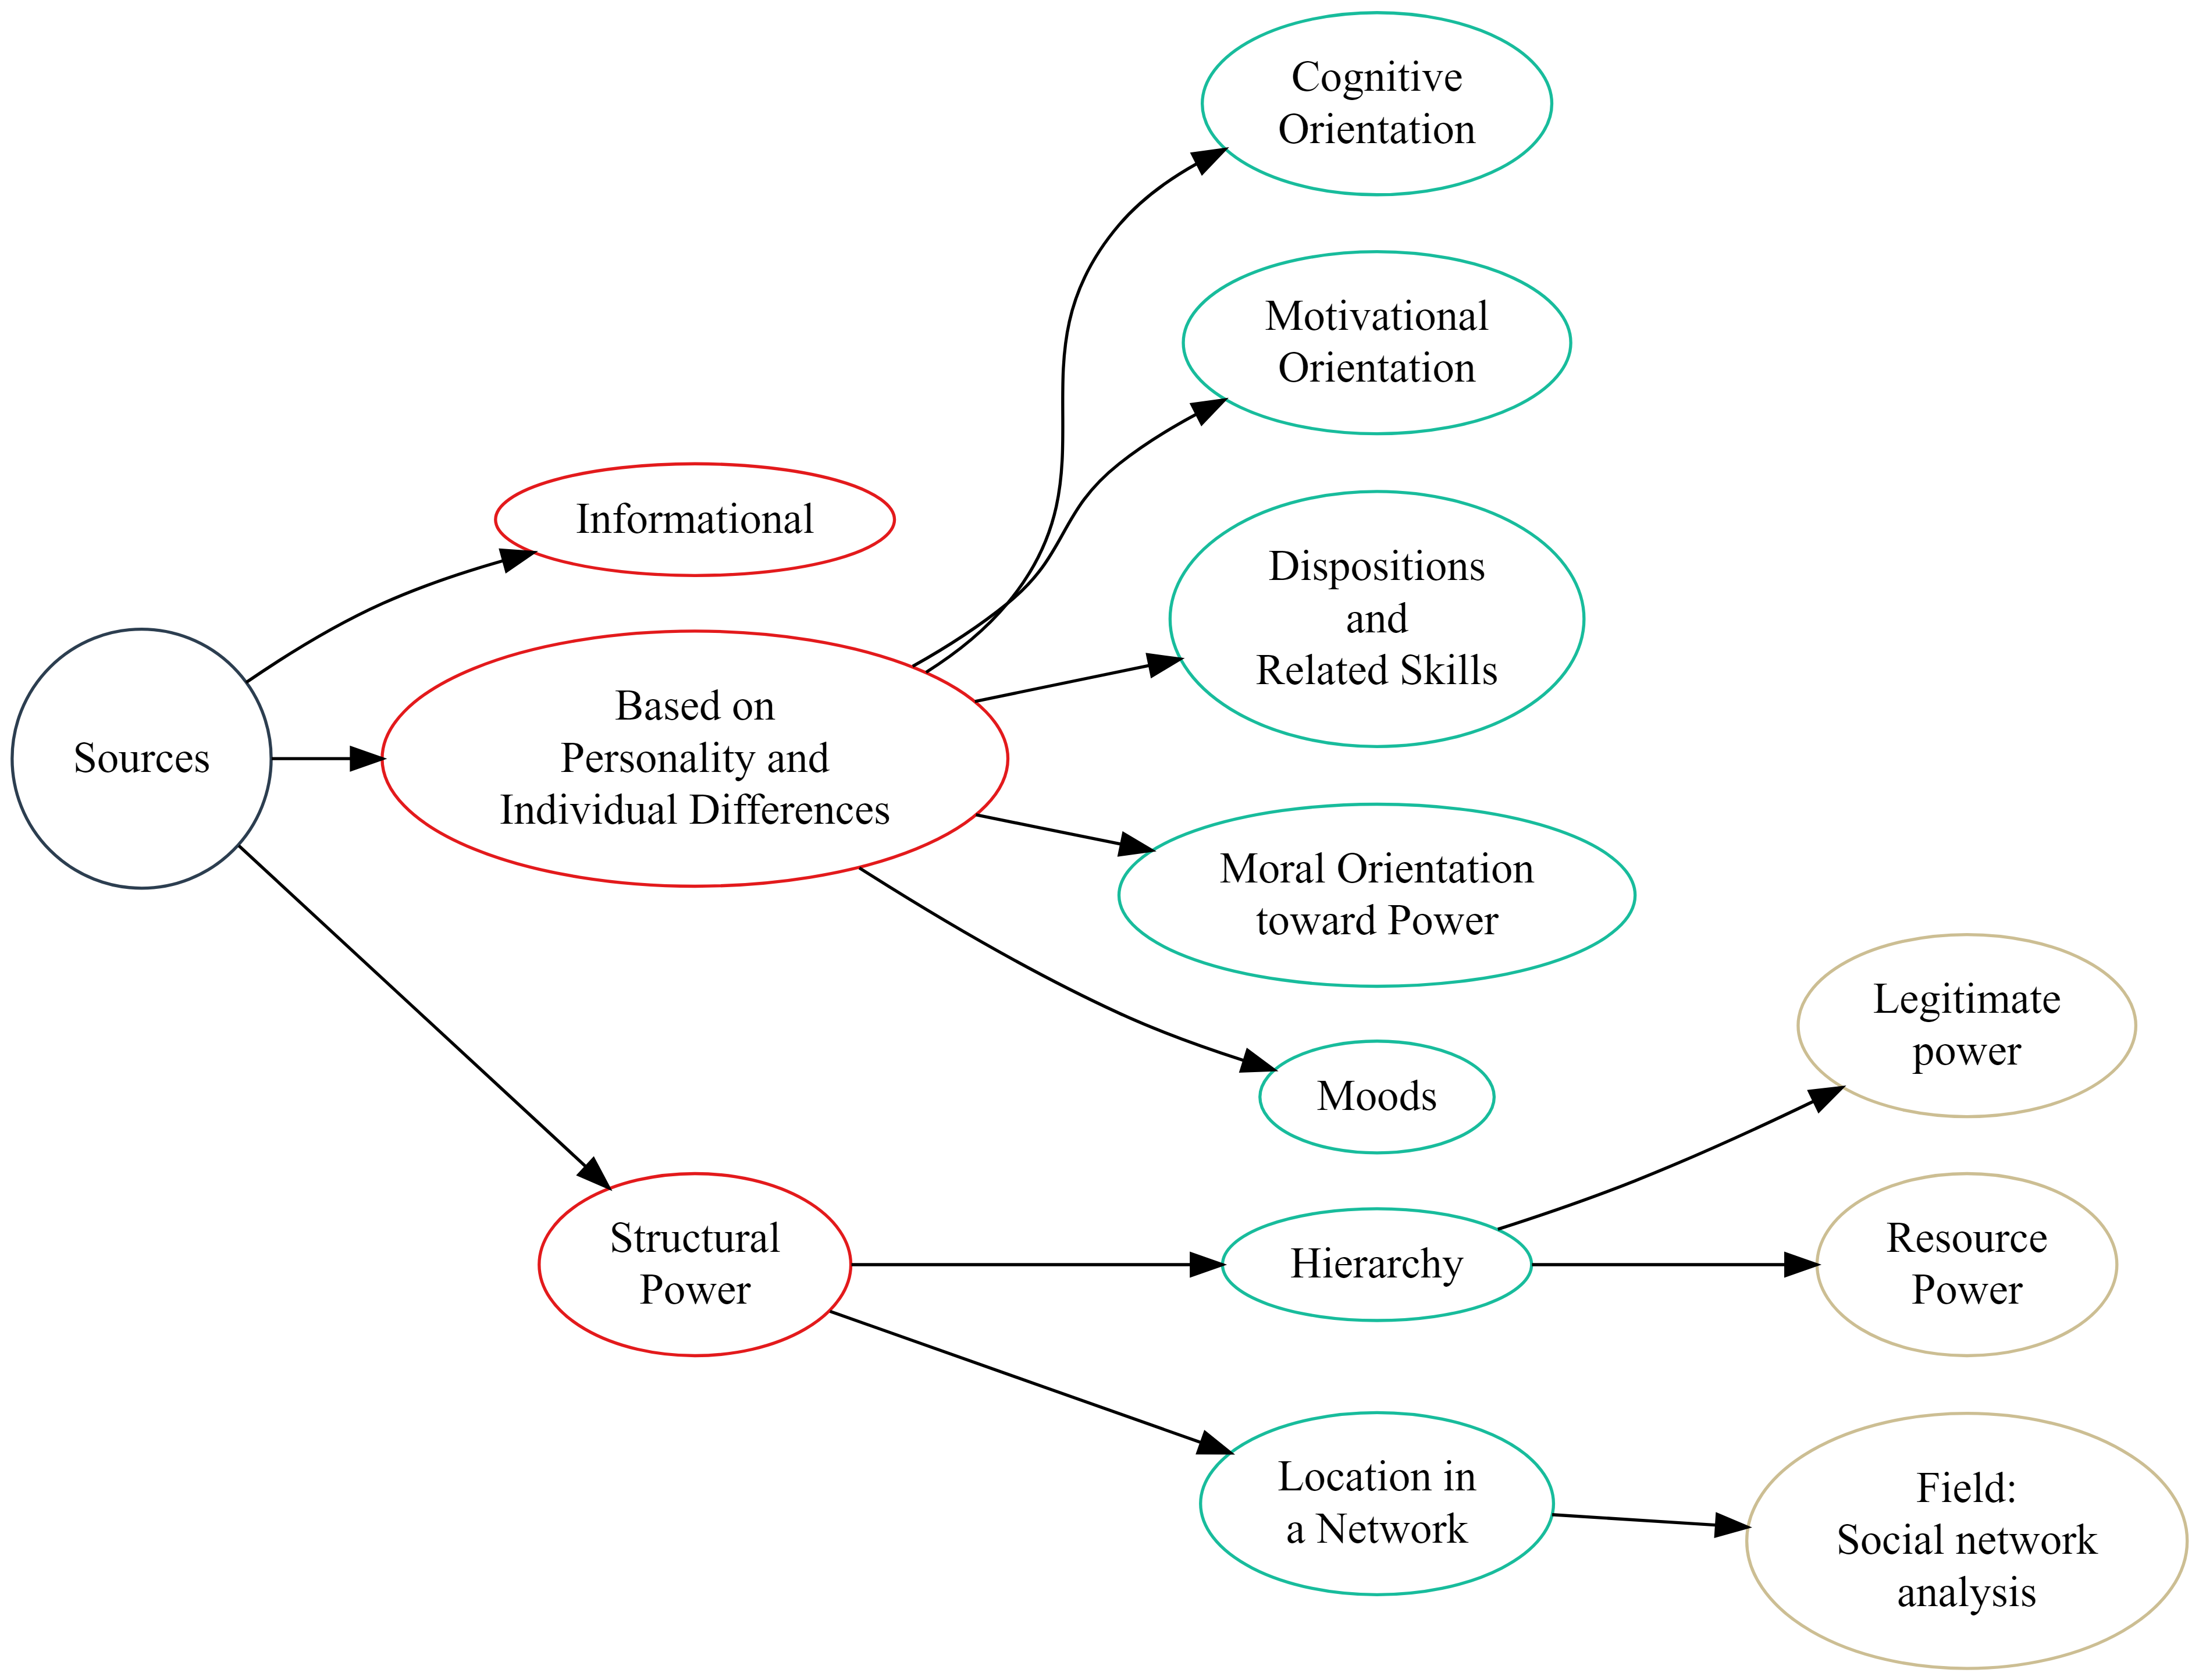
\includegraphics[width=4.5in,height=2.5in]{007_power_files/figure-beamer/dot-figure-4.png}

}

\caption{\label{fig-sources-of-power-1}Sources of power in a negotiation
(\citeproc{ref-lewicki_negociacion_2024}{Lewicki, Barry, and Saunders
2024}, pp 242-260)}

\end{figure}%
\end{frame}

\begin{frame}{}
\phantomsection\label{section-5}
\begin{figure}

\centering{

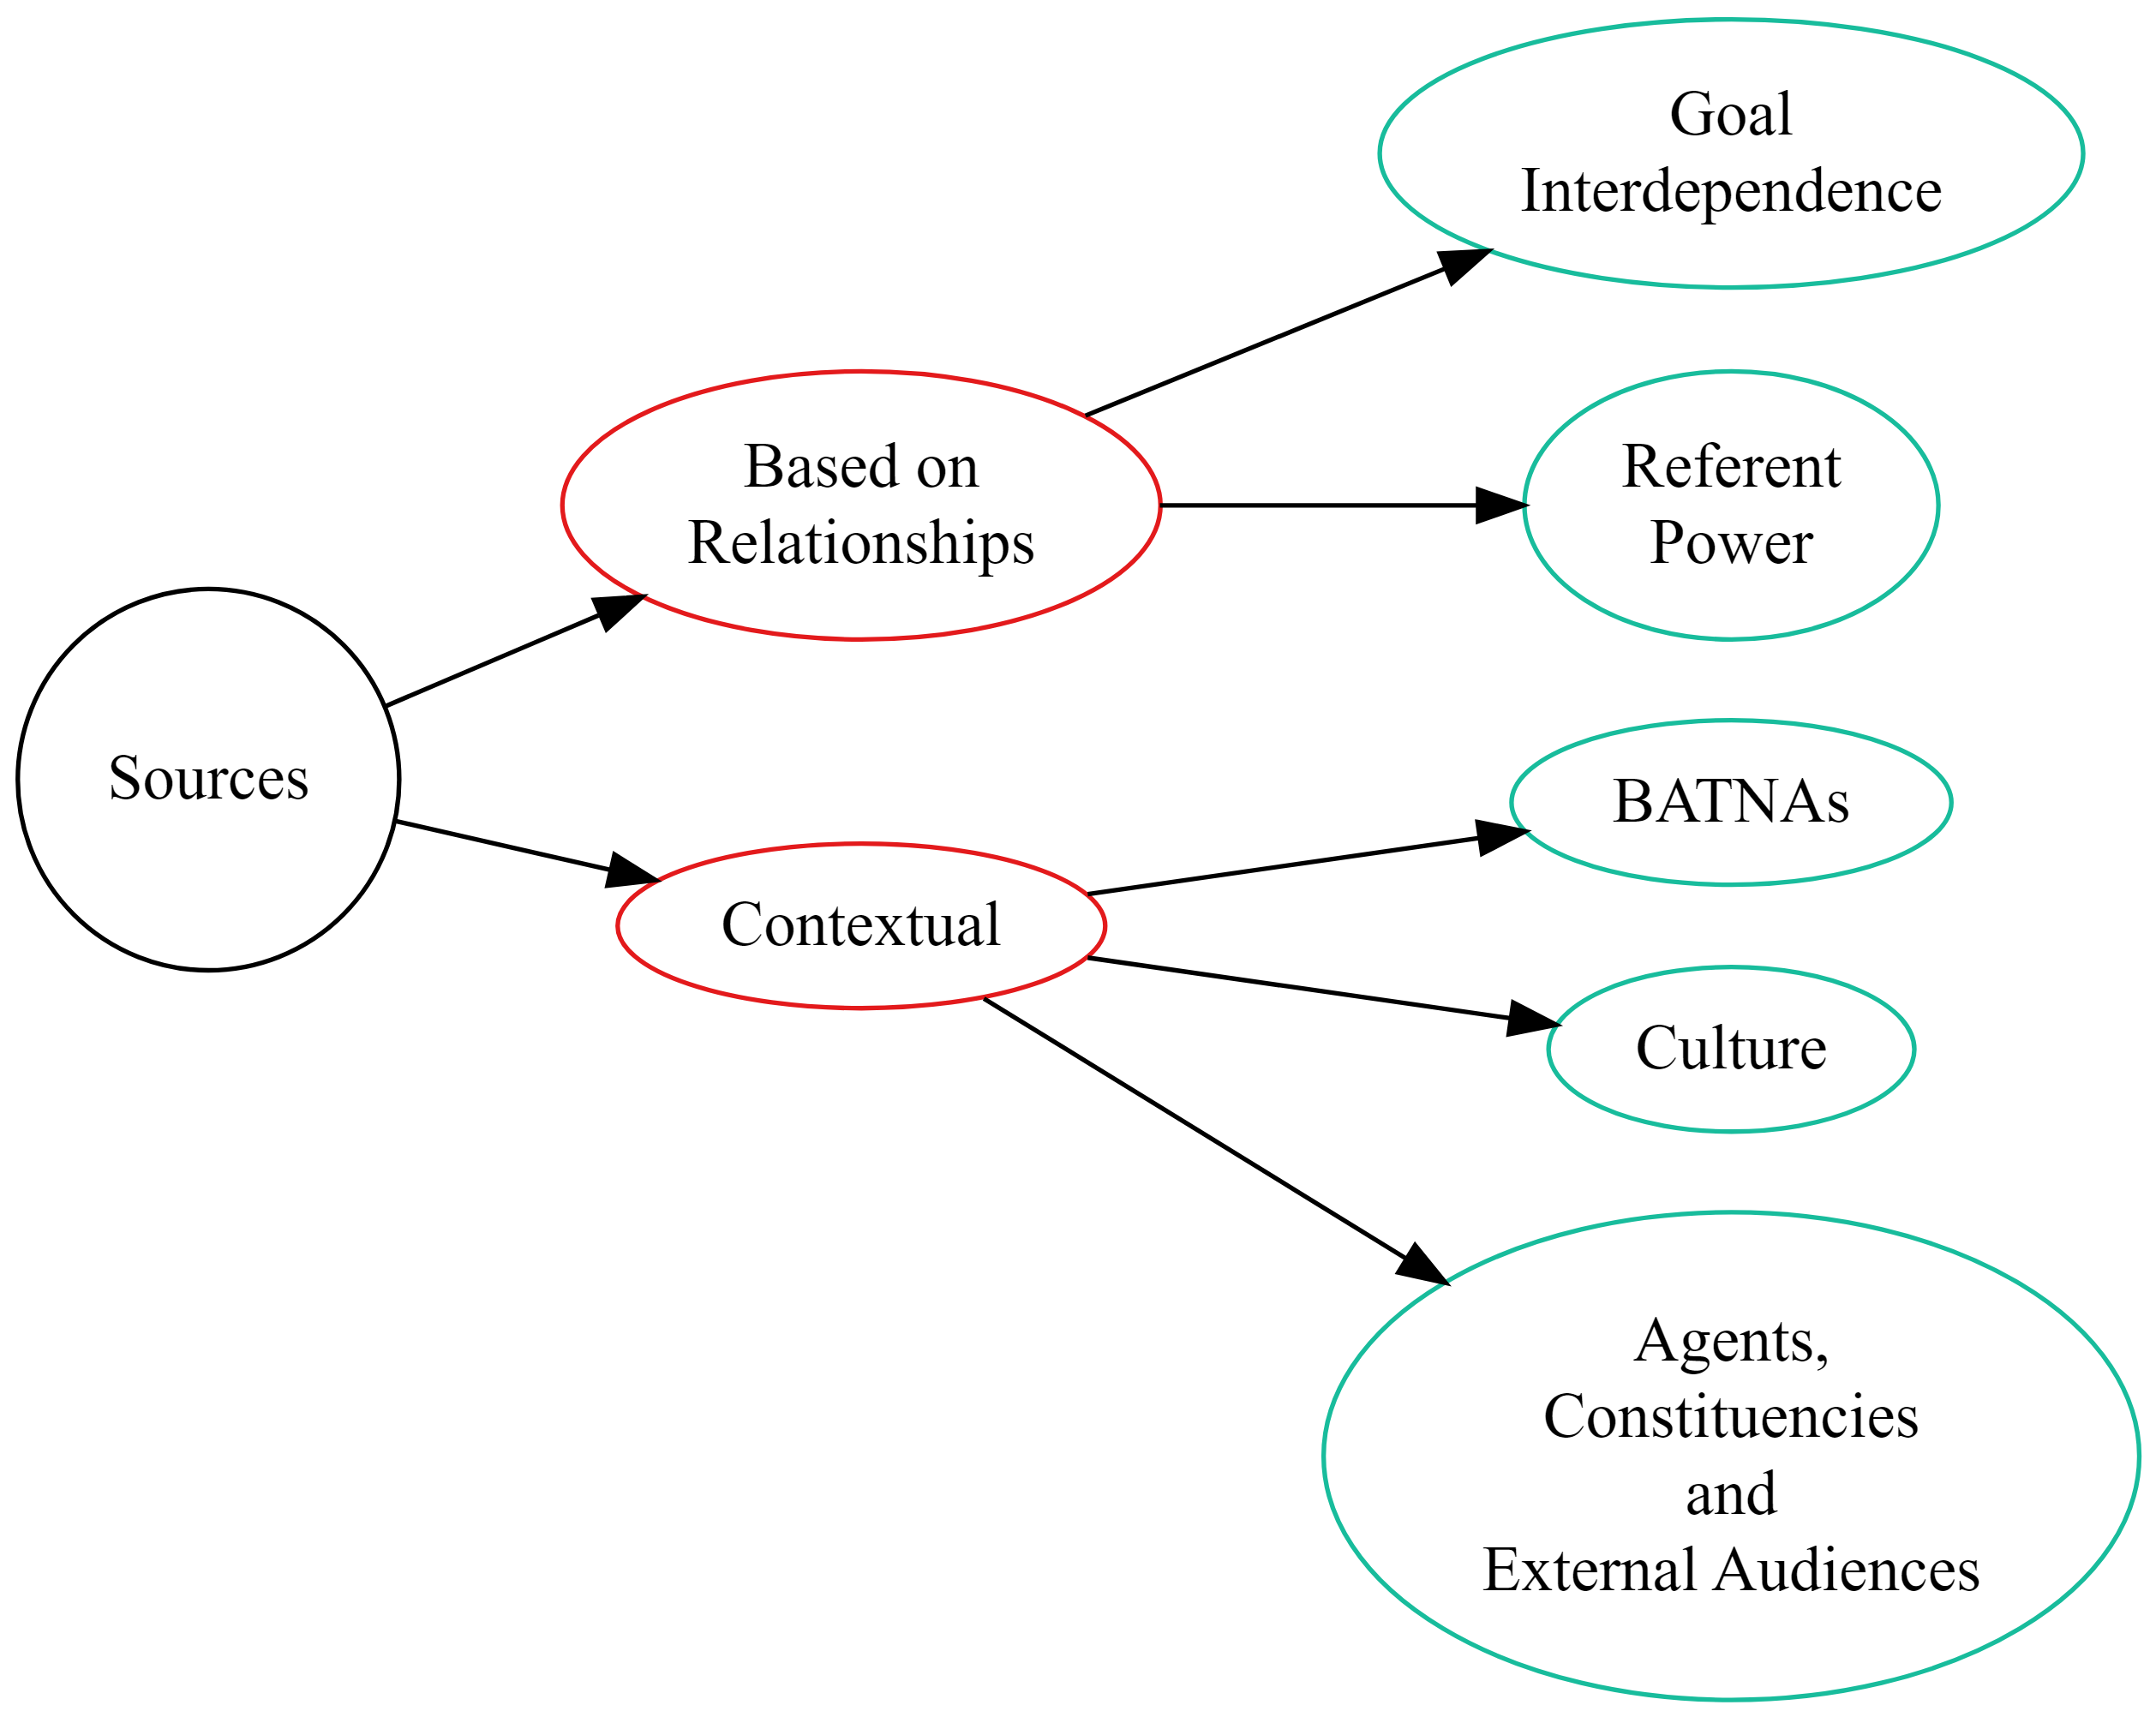
\includegraphics[width=4.5in,height=2.5in]{007_power_files/figure-beamer/dot-figure-3.png}

}

\caption{\label{fig-sources-of-power-2}Sources of power in a negotiation
(\citeproc{ref-lewicki_negociacion_2024}{Lewicki, Barry, and Saunders
2024}, pp 242-260)}

\end{figure}%
\end{frame}

\section{The Consequences of Unequal
Power}\label{the-consequences-of-unequal-power}

\begin{frame}{}
\phantomsection\label{section-6}
\begin{figure}

\centering{

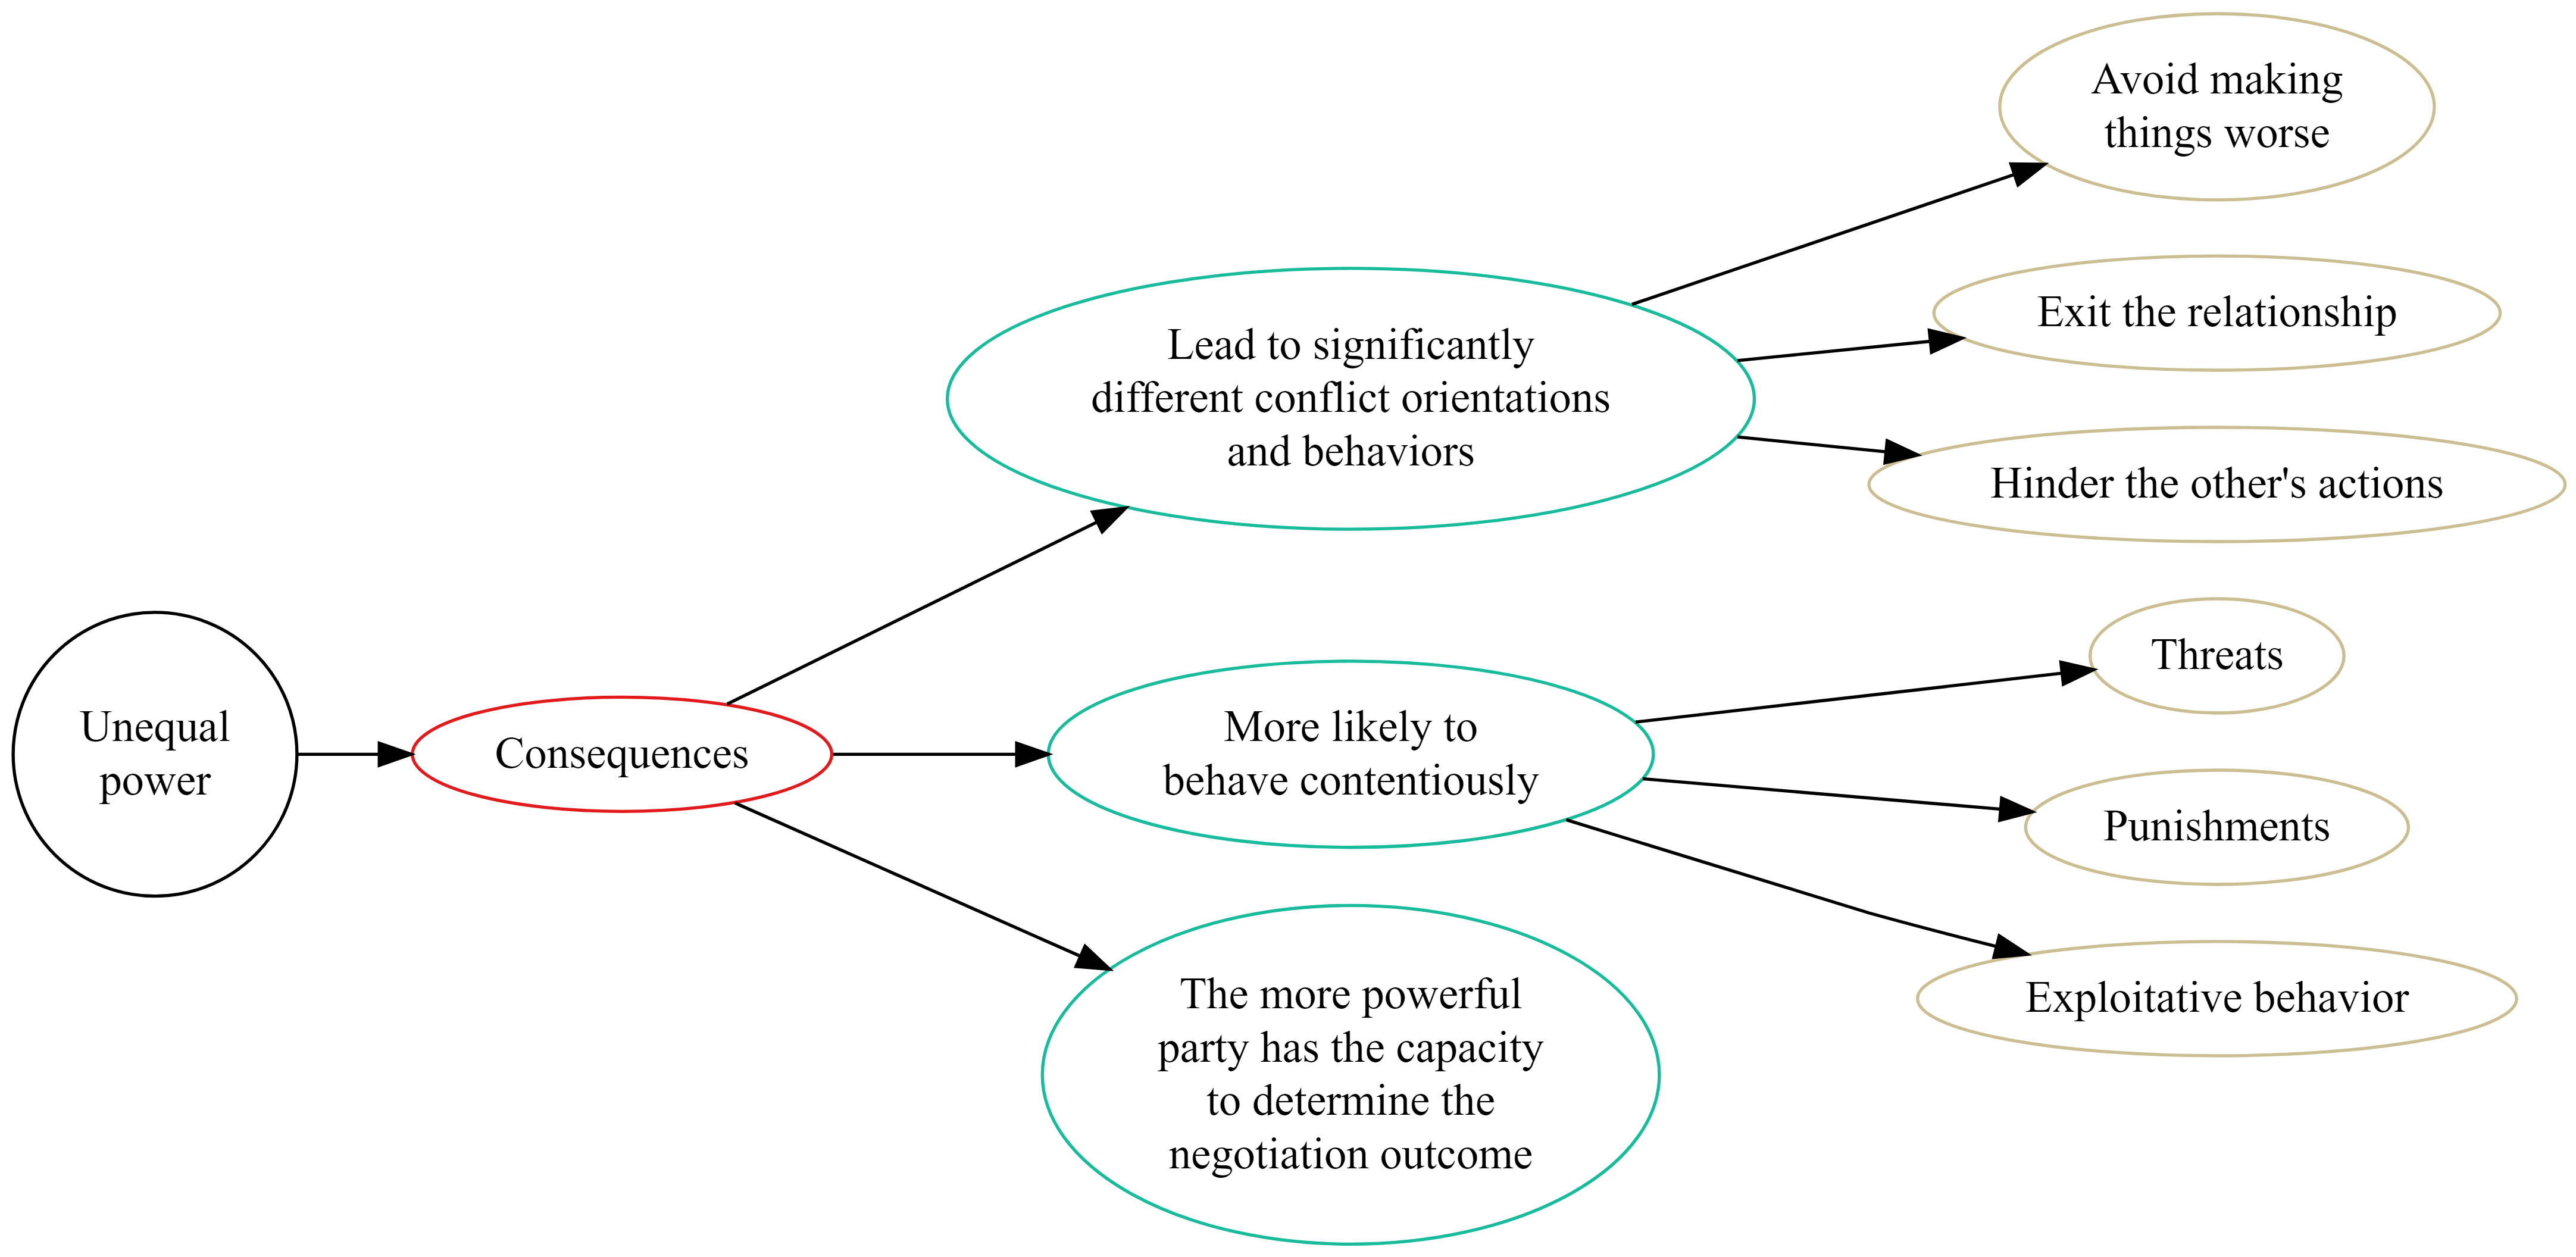
\includegraphics[width=4.5in,height=2.5in]{007_power_files/figure-beamer/dot-figure-2.png}

}

\caption{\label{fig-consequences-of-unequal-power}Consequences of
unequal power in a negotiation
(\citeproc{ref-lewicki_negociacion_2024}{Lewicki, Barry, and Saunders
2024}, pp 260-261)}

\end{figure}%
\end{frame}

\section{Dealing with negotatiors how have more
power}\label{dealing-with-negotatiors-how-have-more-power}

\begin{frame}{}
\phantomsection\label{section-7}
\begin{itemize}
\item
  Advice to negotiators who are in low-power positions based on
  (\citeproc{ref-lewicki_negociacion_2024}{Lewicki, Barry, and Saunders
  2024}, pp 261-262):

  \begin{itemize}
  \tightlist
  \item
    Diversify risk by entering into deals with several other partners.
  \item
    Deal with a variety of different individuals and departments in the
    high-power party (Divide and Conquer).
  \item
    Build coalitions with other low-power players to increase collective
    bargaining power.
  \item
    Enter in early deals with high-power parties and maximize the
    visibility of those deals to other parties.
  \end{itemize}
\end{itemize}
\end{frame}

\begin{frame}{}
\phantomsection\label{section-8}
\begin{itemize}
\item
  Advice to negotiators who are in low-power positions based on
  (\citeproc{ref-lewicki_negociacion_2024}{Lewicki, Barry, and Saunders
  2024}, pp 261-262):

  \begin{itemize}
  \tightlist
  \item
    If you have something to offer, make sure you offer it to more than
    one high-power party to generate competition between them.
  \item
    Gather and leverage relevant information to strengthen your
    negotiation position and achieve better outcomes through persuasive
    communication.
  \item
    Do what you can to manage the process (for example the agenda or
    location) to guide the negotiation towards a more favorable outcome.
  \end{itemize}
\end{itemize}
\end{frame}

\section{Acknowledgments}\label{acknowledgments}

\begin{frame}{}
\phantomsection\label{section-9}
\begin{itemize}
\item
  To my family that supports me
\item
  To the taxpayers of Colombia and the
  \href{https://www.umng.edu.co/estudiante}{\textbf{UMNG students}} who
  pay my salary
\item
  To the \href{https://www.business-science.io/}{\textbf{Business
  Science}} and \href{https://www.rfordatasci.com/}{\textbf{R4DS Online
  Learning}} communities where I learn
  \href{https://www.r-project.org/about.html}{\textbf{R}} and
  \href{https://www.python.org/about/}{\textbf{\(\pi\)-thon}}
\item
  To the \href{https://www.r-project.org/contributors.html}{\textbf{R
  Core Team}}, the creators of
  \href{https://rstudio.com/products/rstudio/}{\textbf{RStudio IDE}},
  \href{https://quarto.org/}{\textbf{Quarto}} and the authors and
  maintainers of the packages
  \href{https://CRAN.R-project.org/package=tidyverse}{\textbf{tidyverse}},
  \href{https://CRAN.R-project.org/package=DiagrammeR}{\textbf{DiagrammeR}},
  \href{https://CRAN.R-project.org/package=knitr}{\textbf{knitr}},
  \href{https://CRAN.R-project.org/package=kableExtra}{\textbf{kableExtra}}
  and
  \href{https://CRAN.R-project.org/package=tinytex}{\textbf{tinytex}}
  for allowing me to access these tools without paying for a license
\item
  To the \href{https://www.kernel.org/category/about.html}{\textbf{Linux
  kernel community}} for allowing me the possibility to use some
  \href{https://static.lwn.net/Distributions/}{\textbf{Linux
  distributions}} as my main
  \href{https://en.wikipedia.org/wiki/Operating_system}{\textbf{OS}}
  without paying for a license
\end{itemize}
\end{frame}

\section*{References}\label{references}
\addcontentsline{toc}{section}{References}

\begin{frame}[allowframebreaks]{References}
\phantomsection\label{refs}
\begin{CSLReferences}{1}{0}
\bibitem[\citeproctext]{ref-coleman_power_2014}
Coleman, Peter T. 2014. {``Power and {Conflict}.''} In \emph{The
{Handbook} of {Conflict} {Resolution}: {Theory} and {Practice}}, 3rd
ed., 137--81. Jossey-Bass.

\bibitem[\citeproctext]{ref-lewicki_negociacion_2024}
Lewicki, Roy J., Bruce Barry, and David M. Saunders. 2024.
\emph{Negociación}. 9th ed. McGraw-Hill Education.
\url{https://www-ebooks7-24-com.ezproxy.umng.edu.co/?il=40562}.

\end{CSLReferences}
\end{frame}




\end{document}
